\documentclass[../../main.tex]{subfiles}
% \documentclass[a4paper,10pt]{ltjsarticle}
\begin{document}
\rhead{京都大学後期$1990$年$6$番}
\setcounter{equation}{0}
\begin{oframed}
  \subfile{problem}
\end{oframed}
\setlength{\columnseprule}{0.4pt}
\begin{multicols}{2}
  {\bf [解答]}

  \paragraph{(1)}
  $X$は$X_i$の和だから
  \begin{align}
    X = \sum_{i=1}^{l} X_i
  \end{align}
  である．  $\cdots$(答)

  \vspace{10pt}
  \paragraph{(2)}
  まず(1)の結果から
  \begin{align}
    X^2 & = \sum_{i=1}^{l} X_i^2 + 2\sum_{i < j} X_i X_j
  \end{align}
  より，期待値は分解できること，および$i\neq j$で$X_i$と$X_j$が独立であることから
  \begin{align}
    E(X^2)
    & = \sum_{i=1}^{l} E(X_i^2) + 2\sum_{i < j} E(X_i X_j)   \\
    & = \sum_{i=1}^{l} E(X_i^2) + 2\sum_{i < j} E(X_i)E(X_j)
  \end{align}
  を計算すれば良い．

  ここで，
  \begin{align}
    E(X_i)   & = \dfrac{1}{n} \\
    E(X_i^2) & = \dfrac{1}{n}
  \end{align}
  を代入すれば
  \begin{align}
    E(X^2) & = \dfrac{\ell}{n} + \dfrac{\ell(\ell-1)}{n^2}
  \end{align}
  である．  $\cdots$(答)

  \vspace{10pt}
  \paragraph{(3)}
  (2)の結果より，
  \begin{align}
    & E(X^2) > 2                         \\
    \iff
    & \dfrac{\ell^2 + (n-1)\ell}{n^2} > 2 \\
    \iff
    & \ell^2 + (n-1)\ell -2n^2 > 0
  \end{align}
  を満たす最小の$l$を求めれば良い．
  \begin{align}
    f(x) = x^2 + (n-1)x -2n^2
  \end{align}
  とおくと，$f(x)=0$の判別式は
  \begin{align}
    D
    & = (n-1)^2+8n^2 \\
    & = 9n^2-2n+1
    > 0
  \end{align}
  であり，$y=f(x)$のグラフの概形は下図である．

  \begin{figure}[H]
    \centering
    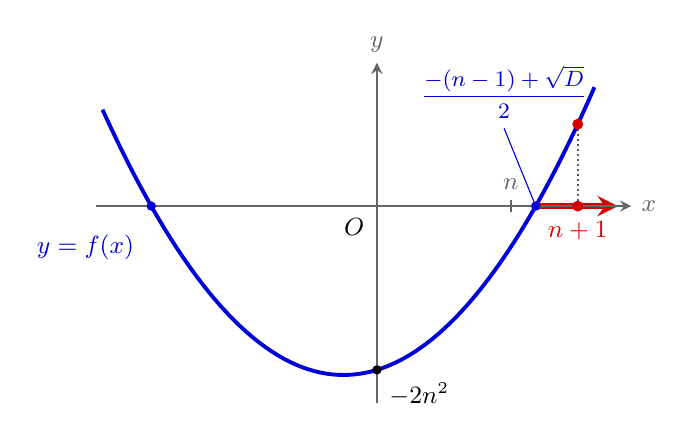
\begin{tikzpicture}[x=0.85cm, y=0.26cm, >=stealth, every node/.style={font=\small}]
      % 図示用に n=2 とする: f(x)=x^2+x-8, 正の根 (-1+sqrt(33))/2 ≈ 2.37 (n < 根 < n+1/2)
      \def\nval{2}
      \pgfmathsetmacro{\rootP}{(-(\nval-1)+sqrt(9*\nval*\nval-2*\nval+1))/2}
      \pgfmathsetmacro{\rootM}{(-(\nval-1)-sqrt(9*\nval*\nval-2*\nval+1))/2}
      \pgfmathsetmacro{\fNext}{(\nval+1)^2+(\nval-1)*(\nval+1)-2*\nval*\nval}

      % f(l)>0 となる範囲 (正の根より右)
      \draw[line width=2.2pt, red!85!black, ->] (\rootP, 0) -- (3.6, 0);

      % 座標軸
      \draw[->, thick, gray!80!black] (-4.2, 0) -- (3.8, 0) node[right] {$x$};
      \draw[->, thick, gray!80!black] (0, -9.6) -- (0, 7) node[above] {$y$};
      \node[below left=1pt] at (0, 0) {$O$};

      % y = f(x)
      \draw[line width=1.4pt, blue!85!black, domain=-4.1:3.25, samples=80]
      plot (\x, {\x*\x+(\nval-1)*\x-2*\nval*\nval});
      \node[blue!85!black, left=2pt] at (-3.4, -2.0) {$y=f(x)$};

      % y 切片 -2n^2
      \node[circle, fill, inner sep=1.2pt] at (0, -2*\nval*\nval) {};
      \node[below right=1pt] at (0, -2*\nval*\nval) {$-2n^2$};

      % 2根
      \node[circle, fill=blue!85!black, inner sep=1.2pt] at (\rootM, 0) {};
      \node[circle, fill=blue!85!black, inner sep=1.2pt] at (\rootP, 0) {};
      \draw[thin, blue!85!black] (\rootP, 0) -- (1.9, 3.8) node[above=0pt, font=\footnotesize, blue!85!black] {$\displaystyle\frac{-(n-1)+\sqrt{D}}{2}$};

      % n と n+1
      \draw[thick, gray!80!black] (\nval, -0.3) -- (\nval, 0.3) node[above=0pt] {$n$};
      \draw[densely dotted, thick, gray!70!black] (\nval+1, \fNext) -- (\nval+1, 0);
      \node[circle, fill=red!85!black, inner sep=1.4pt] at (\nval+1, 0) {};
      \node[below=2pt, red!85!black] at (\nval+1, 0) {$n+1$};
      \node[circle, fill=red!85!black, inner sep=1.4pt] at (\nval+1, \fNext) {};
    \end{tikzpicture}
    \caption{$y=f(x)$ の概形（赤線は $f(x)>0$ となる正の範囲）}
    \label{1990-6:fig:1}
  \end{figure}

  よって，求める$\ell$は
  \begin{align}
    \dfrac{-(n-1)+\sqrt{D}}{2} < \ell
  \end{align}
  を満たす最小の整数である．ここで$n$は自然数だから
  \begin{align}
    0<9n^2-6n+1 < 9n^2-2n+1 < 9n^2
  \end{align}
  の各辺のルートをとって，
  \begin{align}
    3n-1 < \sqrt{D} < 3n
  \end{align}
  なので
  \begin{align}
    n < \dfrac{-(n-1)+\sqrt{D}}{2} < n+\dfrac{1}{2}
  \end{align}
  となり，求める最小の$l$は
  \begin{align}
    \min l = n+1
  \end{align}
  である．$\cdots$(答)

  \vspace{10pt}
  {\bf [解説]}

  \newpage
\end{multicols}
\end{document}
